\section{Dyna}\label{sec:Dyna_experiment}
In the previous section, it was demonstrated that equivariant world models provide advantages over world models without an inductive bias to the symmetries present in the environment.

However, for such techniques to be truly useful, the models must demonstrate an improvement in sample efficiency. This was not the case with the offline trained world models. As the world models required interacting with the MDP many times to create a dataset to learn a model from.

In this section a set agents were trained with online learnt transition models in a full Dyna setting, Alg.\ref{algo:Dyna}. These agents have an actor-critic that non equivariant and then a transition model, which is learnt online. When learnt online the transition models at each Dyna iteration is trained for 100 and 10 epochs for CartPole and Catch, respectively. This ensures that the models are not underfitting, because the same hyperparameters were used to train the offline world models.The next section explores the effects of the equivariant biases in the transition models.

In the same fashion as the Supervised-Dyna agents before, 128 agents were trained at each hyperparameter configuration initialized with independent random seeds. In comparison to the Supervised-Dyna experiments before agents are trained across five planning ratios, $[0.5, 1, 2, 4, 8]$ and $[5, 10, 50, 100]$ Dyna iterations. The planning ratio is the same as before and controls the fraction of time spent planning to acting. The number of Dyna iterations controls the size of the buffer of transitions for both the transition model. To help with reasoning about the training, the size of the replay buffer is:

\begin{equation}
	|\mathcal{D}| = 50000/\text{Num Dyna Iterations}.
\end{equation}
Further, when considering the planning phase, the planning buffer size is related to the acting buffer by the planning ratio:
\begin{equation}
	|\mathcal{D}_p| = \text{PR}|\mathcal{D}|.
\end{equation}
As the number of timesteps is fixed the number of Dyna iterations provides a mechanism for controlling the frequency of planning.
\subsection{Results: CartPole Dyna}
\begin{figure}[h!]
	\centering
	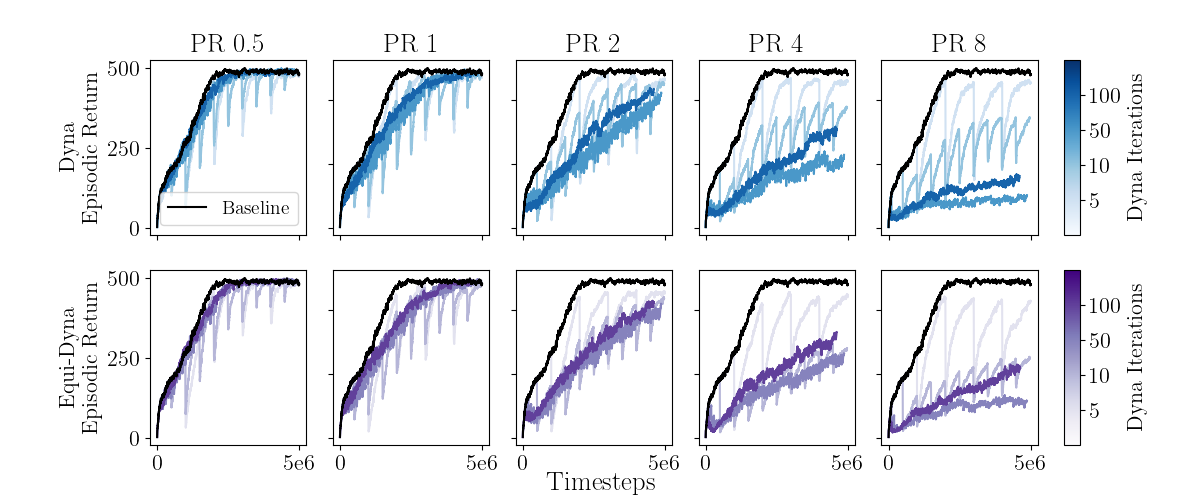
\includegraphics[width=\textwidth]{Figures/dyna_sweep_cp.png}
	\caption{A matrix of plots for mean episodic returns for the CartPole Dyna agents across 128 random seeds
		plotted against number of interaction time-steps in the MDP. The matrix varies planning ratio horizontally, and the top row is the conventional MLP transition model in blue. The equivariant transition models are all on the bottom row, in purple. Each plot contains five lines, in black is the baseline actor-critic implementation. The colorbar indicate the number of dyna iterations used to train the four agents.}
	\label{fig:cp_dyna}
\end{figure}

The matrix of plots in Fig.\ref{fig:cp_dyna} shows underwhelming performance for the Dyna implementation. Both the Dyna and Equi-Dyna agents underperform the baseline actor-critic in all plots. The baseline is the same actor-critic and can be used as a reference point to compare the Dyna and Equi-Dyna implementations. Further, the model's performance is strikingly similar across all planning ratios and Dyna iterations.

When only considering a planning ratio of 0.5, where the agent learns from twice the number of real transitions as simulated transitions, the agents with higher Dyna iteration count, thus fewer gradient updates\footnote{Batch size is constant, so parameter updates is a function of dataset size.} from simulated transitions, perform similarly to the baseline. Additionally, the discontinuities seen in models with higher Dyna iterations were not present.

These discontinuities are caused by the actor-critic network gaining too much experience in the planning environment. If the planning environment does not simulate the true environment well enough.

The evidence for this is threefold. Firstly such discontinuities, are clearly absent in the expert transition model seen in Fig.\ref{fig:sup-dyna-cp}. Where, the pretrained transition model, has access to more data than is seen by the online trained world models throughout the whole training, and achieves much lower validation loss $0.009$ compared with the lowest transition model training loss across all hyperparameters of $0.039$. This fourfold decrease in loss indicates a far more accurate transition model.

Secondly, considering higher planning ratios it can be seen that the discontinuities are even larger. As higher planning ratios correspond to the actor-critic performing more simulated training. This results in further fitting the actor-critic's policy to the simulated environment. When the agent returns to the true environment the return delta is larger for higher planning ratios, indicating an increasingly negative effect on the policy when performing more simulated training.

Finally, when comparing the higher planning ratios at higher Dyna iterations to lower planning rations. One sees that the majority of policy updates are in the simulated environment, and the transition model learns from a limited amount of simulated data. That the effectiveness of the models collapses in the true environment, emphasizing the inability for the policy learnt predominately in the simulated environment to generalize to the true environment.



The lack of differentiation between both the Dyna agents and the Equi-Dyna agents implies that the same issues are present in both. This is attributed to the poor quality of the online learnt world models. Where the equivariant G-CNN transition model's superior data efficiency and generalization is not sufficient to overcome the limited sample count available for training transition models.

\subsection{Catch}
In comparison to the CartPole environment the Catch environment is a small discrete space discrete and may provide a simpler task for learning.
In the same manner as CartPole, a set of experiments were performed which varied the planning ratio and number of Dyna iterations.
\begin{figure}[h!]
	\centering
	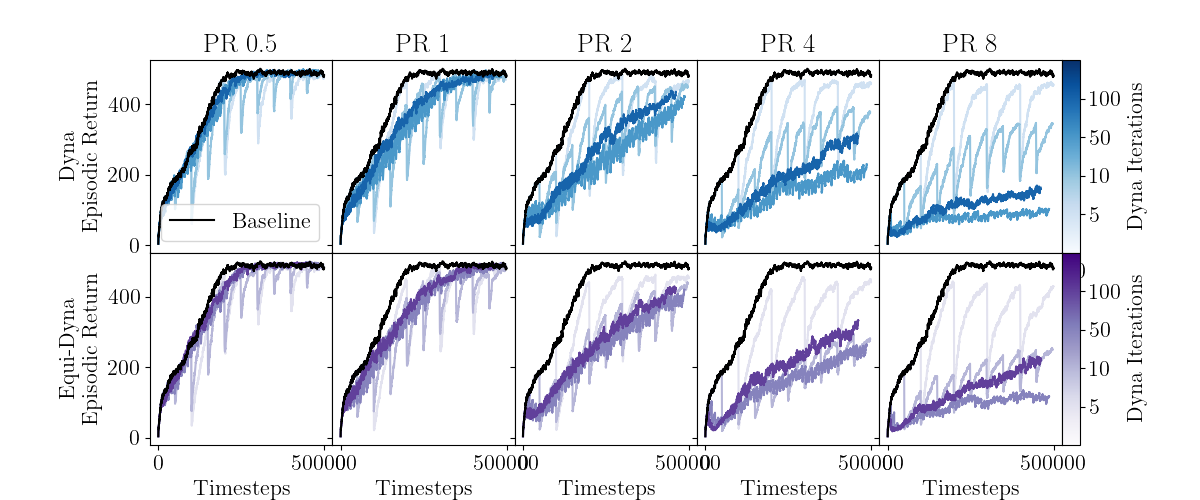
\includegraphics[width=\textwidth]{Figures/dyna_sweep_catch.png}
	\caption{A matrix of plots for mean episodic returns for the Catch Dyna agents across 128 random seeds
		plotted against number of interaction time-steps in the MDP. The matrix varies planning ratio horizontally, and the top row is the conventional MLP transition model in blue. The equivariant transition models are all on the bottom row, in purple. Each plot contains 5 lines, in black is the baseline actor-critic implementation. The colorbar indicate the number of dyna iterations used to train the agents.}
	\label{fig:catch_dyna}
\end{figure}
Despite the small discrete state space, none of the agents were able to improve upon the actor-critic baseline. The similarity, in the patterns shown in the return curves between Catch and CartPole imply that the overfitting to poor simulation is also present.

In the mean returns of the Catch agents over 128 seeds, again minimal difference is seen between the Equi-Dyna agents and the Dyna agents. However, their training dynamics do seem to be similar. At higher iteration count, the return curves are smoother due to a reduced number of updates in the planned environment not allowing the policy to drift from the value learnt in the true environment. When the planning ratio is increased, the impact upon the quality of the policy is more severe. This degradation is attributed to overfitting the policy to an insufficiently accurate simulated environment.

In comparison to CartPole, the Catch environment only has 675 possible transitions. However, when testing the expert policy and the random policies in Section~\ref{sec:model-based} the joint expert random policy, did not sample every possible state action pair, in 10,000 sampled transitions. When training the agent's world model online from the replay buffer, not all transitions may be present, and the model's inability to generalize to unseen states is still a problem. This poor generalization performance is clear in the return curves as the agent's transition models are not able to produce sufficiently accurate transitions for the policy to learn from.


\section{Conclusion}
In both environments similar behaviour was observed. The Dyna and Equi-Dyna have very comparable performance at the same hyperparameters, which always underperformed the baseline. As such, planning with online models was ineffective.

The poor performance was attributed to transition models that do not deliver sufficient accuracy in producing trajectories that simulate the environment well enough to provide an alternative to samples in the true environment.

The inaccurate transition models suggest providing the models with more data and/or not using the transition model before some point in the training such that enough data can be sampled from the MDP that the transition model can generalize effectively. This however, would not have been straightforward to implement. Implementation constrains of the numerical computing library JAX and available memory, meant that there was no ability to grow array size in code compiled to the XLA backend. This in conjunction with the large memory footprint of thousands of transitions, meant that the workarounds tried with pre allocated replay buffers were infeasible due to out of memory errors on the GPU and RTX 3090.

